% !TEX root = ../Dissertation.tex
%===================================================================================================

\chapter{Materials and Methods}



\section{Mice}
\label{methods:mice}

NOD, NOD.$\mu$MT\textsuperscript{-/-}, NOD-RAG2p-GFP, NOD.$\mu$MT\textsuperscript{-/-}.RAG2p-GFP and C57BL/6 (B6) mice were used.

NOD.$\mu$MT\textsuperscript{-/-} (hereafter referred to as NOD KO) mice are deficient in B cells and have been described elsewhere \citep{Serreze1996}.
They have a mutation in their IgM heavy chain which prevents heavy chain rearrangement and subsequent progression from the pro B cell stage to the pre B cell stage.
This block in development results in an inability to produce mature B cells and antibody secreting plasma cells.

RAG2p-GFP reporter mice on a FVB background have also been described elsewhere \citep{Yu1999}.
RAG2p-GFP reporter mice express green fluorescent protein (GFP) under the control of the RAG promoter so that when RAG is expressed, so is GFP.
When RAG transcription is deactivated, so is GFP transcription.
However, the protein decays over time with a half life of ~56 hours \citep{McCaughtry2007}, meaning that GFP\textsuperscript{+} cells can be seen even after RAG deactivation.

For use in this project, FVB-RAG2p-GFP mice were backcrossed 12 generations (N12) to the NOD mouse to produce NOD-RAG2p-GFP reporter mice (hereafter referred to as NOD-RAG-GFP mice).

NOD.$\mu$MT\textsuperscript{-/-}-RAG2p-GFP reporter mice (hereafter referred to as NOD KO-RAG-GFP mice) were also used in this project.
For this, N12 NOD-RAG2p-GFP mice were crossed with NOD.$\mu$MT\textsuperscript{-/-} mice.
Heterozygous progeny were then crossed back to NOD.$\mu$MT\textsuperscript{-/-} mice.
Mouse genotypes were determined by flow cytometric analysis of blood samples to assess IgM and/or GFP presence.

All mice were housed in specific-pathogen-free barrier conditions at York University Biological Services Facility. 
All experimental procedures were conducted under U.K. Government Home Office guidelines.
For mouse studies, investigations were carried out double or single blind, as stated in results, following ARRIVE guidelines \citep{Arriveguidelines}


\section{Cell preparation}
\label{sec:cellprep}

\subsection{Preparation from frozen tissue}

Frozen immune cells housed at -80 \textdegree C in the Green Lab biobank, were quickly defrosted by incubation in a waterbath at 37 \textdegree C.
Defrosted cells were immediately resuspended in 5 mL phosphate buffered saline (PBS) supplemented with 0.5\% bovine serum albumin (BSA) (hereafter referred to as 0.5\% PBS/BSA) and transferred to 15 mL tubes.
Cells were then centrifuged for 3 minutes at 1200 revolutions per minute (rpm), supernatant discarded and the washing step was repeated once more to ensure complete removal of the solution the cells had been frozen in.
The cells were then resuspended in 2 mL 0.5\% PBS/BSA and put in incubator at 37 \textdegree C, 5\% CO2 \todo{subscript} for 2 hours to enable re-expression of cell-surface molecules that had been downregulated due to the freezing process.
Cells then centrifuged as before, supernatant discarded and cells resuspended in a volume appropriate for the subsequent procedure they were to be utilised in.

\subsection{Preparation from fresh tissue}
Freshly prepared cells were isolated from the thymus, spleen, inguinal lymph nodes, pancreatic lymph nodes and bone marrow.
For preparation of bone marrow cells, the femur and tibia were isolated and tissue gently removed using a razor, leaving clean bone.
The cells were isolated by flushing of femur and tibia of mouse with 1 x PBS.
For thymi and spleens, harvested tissues were homogenised using a seive and 2 mL syringe plunger.
Lymph nodes were isolated and placed in a petri dish containing 5 mL PBS.
The cells were liberated by grinding the tissue between two frosted glass slides.
The cell suspensions were centrifuged for 3 minutes at 1200 rpm to pellet cells then the supernatant was discarded.
Where appropriate, red blood cells were lysed by resuspending cells in 1 mL of water for 6 seconds, followed by 1 mL 2 x PBS to neutralise toxicity of the water.
The cells were then centrifuged as before, supernatant discarded and the cells were resuspended as appropriate for subsequent procedure.

\section{Flow cytometry}

Single cell suspensions were prepared as in \cref{sec:cellprep} and the cells were resuspended in 1 mL of 1 x PBS.
100 $\mu$L of cell suspension (equvalent to 10\textsuperscript{6} to 10\textsuperscript{7} cells) was then transferred to an appropriate vessel.
The cells were incubated with 1:300 dilution of anti-CD16/32 antibody and incubated for at least 10 minutes at 4 \textdegree C.
This was carried out to block Fc receptors to avoid non specific antibody binding of analytic antibodies used in the subsequent staining.
The cells were then stained using appropriate fluorescently labelled antibodies and incubated for 25 minutes at 4 \textdegree C in the dark.
Antibodies (from eBioscience or BD Pharmingen) were used at 1:300 dilution, apart from anti-CD4 and anti-CD8 antibodies which were used at 1:800 dilution. 
The cells were washed in 3 mL 1 x PBS and centrifuged for 3 minutes at 1200rpm to remove unbound antibodies.
The supernatant was discarded then the cells were resuspended in 500 $\mu$L of 1 x PBS.

If biotin-conjugated antibodies were used, the dilution, incubation and washing steps were conducted as above.
Subsequently, fluorescent-labelled streptavidin was added at 1:800 dilution in 1 x PBS and incubated for 20 mins at 4 \textdegree C.
Unbound streptavidin was removed by washing with 3 mL of 1 x PBS as above and the cells were resuspended in 500 $\mu$L of 1 x PBS.


\textbf{All antibodies used in this study were assessed and optimised for use against isotype controls}

Data was acquired on a Dako CyAn\texttrademark  Flow Cytometer using Summit software and analysed using FlowJo software.

Antibody clones and suppliers are shown in \cref{fig:antibodyclones}. \todo{Check purified antibody clones, CD25, SA and other CD8 antibodies}

\begin{table}
\caption{Antibody clones and suppliers}
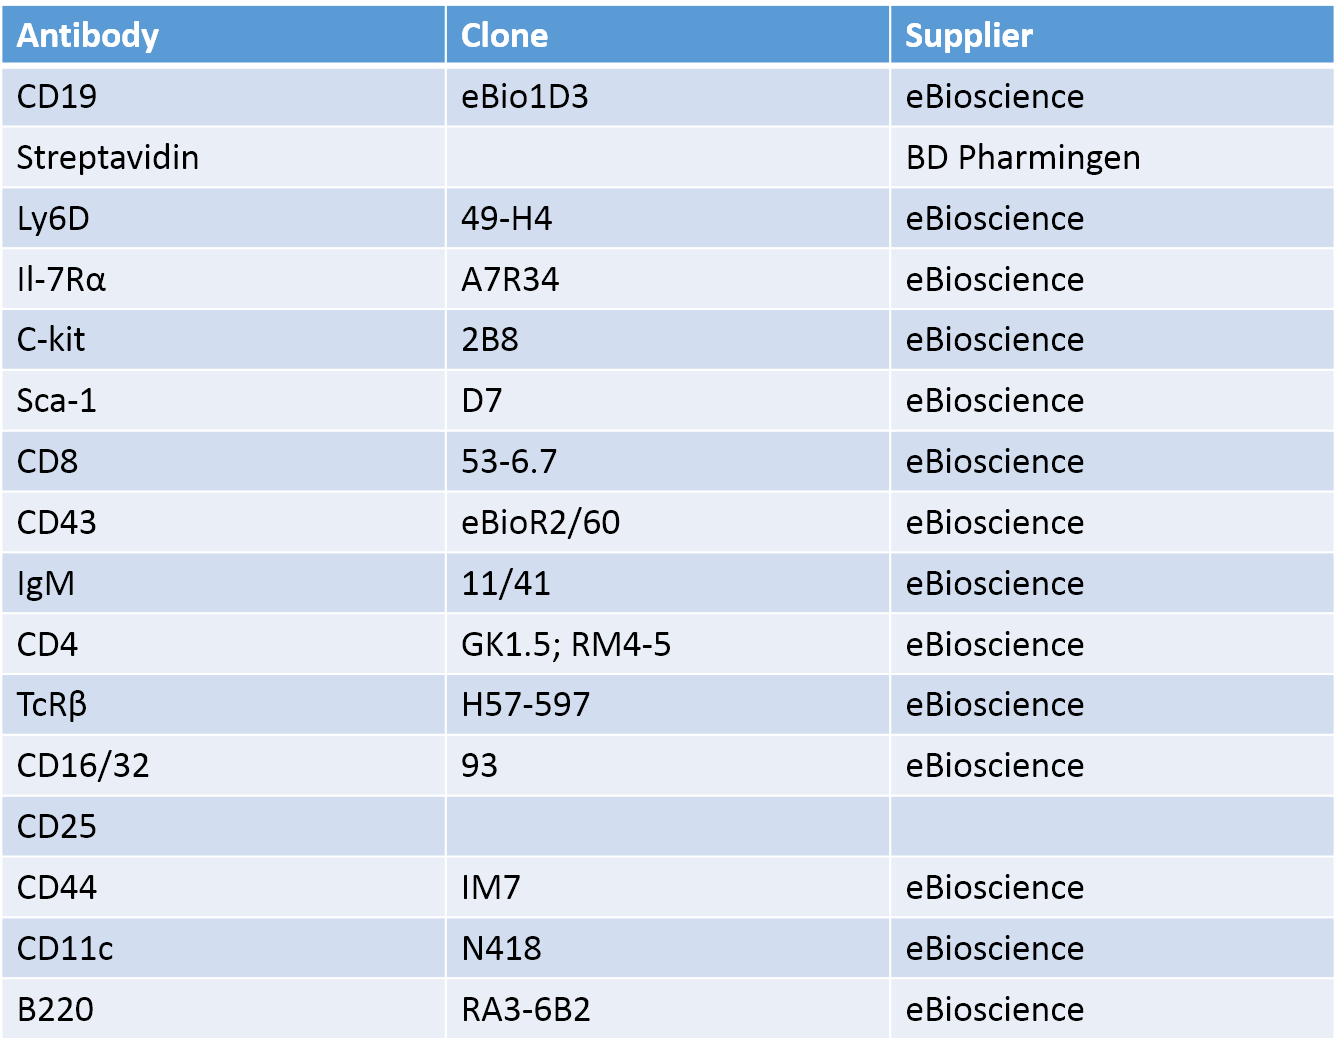
\includegraphics[width=\textwidth]{Figures/Antibodyclones.png}

\label{fig:antibodyclones}
\end{table}

\section{Magnetic cell sorting}
\label{Methods:MACSdepletion}

\subsection{Miltenyi beads and columns}
\label{subsec:Miltenyibeads}

The cells were prepared as in \cref{sec:cellprep}.
For a cell lineage depletion, lineage cell depletion kit (Miltenyi Biotech) was used.
For separation of samples into CD19\textsuperscript{+} and CD19\textsuperscript{-} fractions, CD19 microbeads (Miltenyi Biotech) were used.
For both lineage depletion and CD19 separation, Miltenyi LS columns were used. %and the maufacturers protocols were followed.
There were two deviations from the manufacturers protocol.
Firstly, the addition of an Fc receptor-blocking step prior to the addition of the beads using anti-CD16/32 antibody at 1:300 dilution.
Secondly, the buffer used was 0.5\% PBS/BSA, rather than the buffer suggested in the protocol.
Purity of the appropriate cells was verified by flow cytometric analysis.
The cells were resuspended in a volume of buffer appropriate for the procedure that they were to be used in.

\subsection{Qiagen BioMag goat anti-rat IgG beads}

Cells were prepared as in \cref{sec:cellprep}, resuspended in 500 $\mu$L of 0.5\% PBS/BSA.
A 1:300 dilution of anti-CD16/32 antibody was added and samples were incubated at 4 \textdegree C for 10 minutes to block Fc receptors.
The cells were then incubated with the appropriate purified antibodies depending on which cell populations were to be depleted.
Antibodies were added at \todo{Dilution} dilution and incubated for 20 minutes at 4 \textdegree C.
1 mL \todo{Number of beads} BioMag goat anti-rat IgG beads (Qiagen) were transferred to a 15 mL tube and 10 mL PBS was added.
The solution was placed on a magnet and left for ~10 minutes to allow the beads to adhere.
A pasteur pipette was used to remove the supernatant and the beads were resuspended in 500 $\mu$L of PBS.
The beads were put back on the magnet and allowed to adhere again before removing supernatant as before.
A final wash in 500 $\mu$L PBS performed then beads finally resuspended in 500 $\mu$L PBS.

The cells were prepared by washing in 3 mL PBS and centrifuging for 10 minutes at 1200 rpm.
The cell pellet was then resuspended with the 500 $\mu$L solution of beads and incubated for 15 minutes at 4 \textdegree C.

The samples were then placed on a magnet and beads allowed to adhere.
Supernatant containing unbound cells were removed with clean pasteur pipette, kept, and put back on magnet to remove residual beads.
The cellular supernatant was isolated as before and centrifuged for 3 minutes at 1200rpm.
The cells were then resuspended in 500 $\mu$L 1 x PBS for subsequent flow cytometric analysis.

\section{RNA preparation}

Cells were prepared as in \cref{sec:cellprep}, then RNA extracted using RNeasy mini kits (Qiagen) following the maunufacturers protocol.
A DNAse step was included where deoxyribonuclease I (Sigma) was added to column membrane for 10 minutes at room temperature.
The addition of a DNAse step was to prevent the binding of primers to residual genomic DNA.
%improved the clarity of bands of products on gel electrophoresis following PCR by removing residual genomic DNA.
RNA quality was assessed on the NanoDrop (ThermoScientific NanoDrop 2000), with the aim of producing RNA with 260/280 and 260/230 values of near to, or above, 2.0 which indicates a good purity of RNA.
RNA was resuspended in RNAse-free water and stored at -80 \textdegree C.


\section{Reverse transcription of RNA to cDNA}

RNA was reverse transcribed to cDNA using Superscript II reverse transcriptase (Invitrogen, 2000 U/$\mu$L).
\todo{how much RNA?} RNA was taken and heated at 55 \textdegree C for 10 minutes before being placed on ice.
7 $\mu$L of first buffer (4 $\mu$L 5 x 1st strand buffer (Invitrogen), 2 $\mu$L 10mM dNTP mix (Thermo Scientific), 1 $\mu$L OligodT 0.5 $\mu$M (Invitrogen)) was added to 10 $\mu$L of RNA and the solution was placed in RNAse-free PCR strips.
Amount of RNA was normalised across samples using data from NanoDrop in order to try and keep quantities of cDNA constant across samples.
The volume was then made up to 10 $\mu$L by the addition of RNAse-free water.
The samples were then incubated at 65 \textdegree C for 5 minutes to uncoil RNA, then cooled quickly on ice.
Three $\mu$L of a second buffer (1 $\mu$L 0.1M DTT, 1 $\mu$L RNAse out, 1 $\mu$L Superscript II (all Invitrogen) was then added to each sample and the solution incubated at 65 \textdegree C for 45-60 minutes to make cDNA.
cDNA was stored at -20 \textdegree C until needed.

\section{Primer design}

Specific primers for polymerase chain reaction (PCR) to look for B cell development genes were designed using sequences derived from the National Center for Biotechnology Information (NCBI) nucleotide database \citep{NCBIdatabase} then looking for suitable primers for these genes using Primer3 (www.primer3.ut.ee) \citep{Primer3}.
The primers were then put through a primer blast \citep{Primerblast} to check for specificiy for the desired gene. \todo{Confidence?}
Designed primers (obtained from Sigma Genosys) were then tested to find their optimum annealing temperature by carrying out a temperature gradient PCR from 52-62 \textdegree C.
%This also checked that all primers were working, shown by a band at the expected product size when PCR products were run on a gel.

Primers are as follows:
\begin{itemize}
\item E2A. Forward TTG ACC CTA GCC GGA CAT AC.
Reverse TGC CAA CAC TGG TGT CTC TC.
Expected product size: 150bp.
Optimum annealing temperature: 61.8 \textdegree C.

\item EBF.
Forward CAG TTC TGC AAA GGG ACA CC.
Reverse CAA TGT CGG CAG CTC TCT TC.
Expected product size:226 bp.
Optimum annealing temperature: 59.4 \textdegree C.

\item Pax5. Forward AAC TTG CCC ATC AAG GTG TC.
Reverse CTG ATC TCC CAG GCA AAC AT.
Expected product size: 217bp.
Optimum annealing temperature 61.3 \textdegree C.

\item VPreB.
Forward CGA TAT CCC ACC TCG CTT CT.
Reverse CCG AGC AAA GCA AAC TCT GT.
Expected product size: 238 bp.
Optimum annealing temperature: 59.4 \textdegree C.

\item CXCL12.
Forward GCT CTG CAT CAG TGA CGG TA.
Reverse TAA TTT CGG GTC AAT GCA CA.
Expected product size: 184 bp.
Optimum annealing temperature: 60.5 \textdegree C.
\end{itemize}

\section{Polymerase chain reaction}

Non quantitative polymerase chain reaction (PCR) was carried out to look for the genes of interest using the primers outlined above.
PCR samples consisted of 1 $\mu$L cDNA, 1.125 $\mu$L forward primer, 1.125 $\mu$L reverse primer, 2.5 $\mu$L 25 mM MgCl{2} (Applied Biosystems), 2.5 $\mu$L 25 mM Amplitaq360 buffer (Applied Biosystems), 15.5 $\mu$L dH{2}O, 0.125 $\mu$L 250 U AmpliTaq 360 DNA Polymerase (Applied Biosystems).
cDNA was amplified following 35 cycles of 1 minute at 94 \textdegree C, 1 minute at the appropriate annealing temperature for the primer set, 1 minute at 72 \textdegree C. 
A final elongation step of 10 minutes at 72 \textdegree C was performed once at the end of the 35 cycles.
Amplified cDNA was subsequently analysed by gel electrophoresis.

\section{Gel electrophoresis}

Gel electrophoresis of PCR products were carried out using 3\% agarose gels (Lonza SeaKem LE Agarose) made in 1 x Tris acetate-EDTA (TAE) buffer (Sigma) supplemented with 1 $\mu$L of 10 mg/mL ethidium bromide (\todo{EtBr supplier}) per 25 mL TAE buffer.
5 $\mu$L of 6x loading dye \todo{Supplier loading dye} were added to each 25 $\mu$L PCR product sample.
Total volume of 30 $\mu$L was then transferred to wells in the gel, held in a gel rig containing 1 x TAE buffer.
100 base pair (bp) ladder also put in a well of the gel to show size of bands seen in the gel.
Gels were run at constant 70 Volts until bands had separated sufficiently and imaged using SynGene software.

\section{Statistical Analyses}

All graphs were drawn using GraphPad Prism and statistical analyses (One way ANOVA, Tukey's tests and Mann-Whitney tests) were performed using built-in functions within the software.
